\documentclass[fleqn]{beamer}

\mode<presentation> {
\usetheme{Madrid}
\usecolortheme{dolphin}
}

\usepackage[utf8]{inputenc}
\usepackage[brazilian]{babel}
\usepackage{amsmath}
\usepackage{amssymb}
\usepackage{booktabs}
\usepackage{listings}
\usepackage{xcolor}
\usepackage{tikz}
\usepackage{graphicx}

\lstset{
	basicstyle=\ttfamily\scriptsize,
	breaklines=true,
	keywordstyle=\color{blue!60!black},
	commentstyle=\color{gray},
	stringstyle=\color{green!45!black},
	showstringspaces=false,
	columns=fullflexible,
	frame=single,
	framesep=4pt,
	aboveskip=6pt,
	belowskip=2pt,
}

\title[Aula 6 -- Complexidade e Heurísticas]{Complexidade Computacional, P versus NP e Heurísticas}
\subtitle{Da formulação exata à heurística: o caso do TSP}
\author[Santi]{Prof. \'Everton Santi}
\institute[UFRN/ECT]{ECT2524 -- Introdução à Otimização \\ Escola de Ciências e Tecnologia -- UFRN}
\date{Aula 6}

\begin{document}

\begin{frame}
	\titlepage
\end{frame}

\begin{frame}
	\frametitle{Sumário}
	\tableofcontents
\end{frame}

%------------------------------------------------------------
\section{Motivação}
%------------------------------------------------------------

\begin{frame}
	\frametitle{Um cenário}
	\begin{itemize}
		\item Seu chefe pede uma rota de entregas, calculada em um
			computador comum, com poucos gigabytes de memória e poucos
			minutos de processamento;
		\item O problema é um TSP de porte moderado — algumas centenas de
			cidades;
		\item A formulação exata está correta, mas o solver não termina
			dentro do tempo e da memória disponíveis;
		\item Você não conseguiu resolver o problema. Seu chefe quer
			saber por quê. Qual resposta você dá?
	\end{itemize}
\end{frame}

\begin{frame}
	\frametitle{Três respostas possíveis}
	\begin{itemize}
		\item Há, essencialmente, três respostas possíveis a essa
			pergunta — cada uma com uma força de justificativa muito
			diferente (Garey \& Johnson, 1979).
	\end{itemize}
\end{frame}

\begin{frame}
	\frametitle{Resposta 1 --- ``Não consegui, sou ruim nisso''}
	\begin{center}
		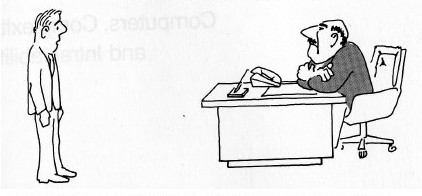
\includegraphics[width=0.55\textwidth]{images/chefe1.jpg}
	\end{center}
	\begin{itemize}
		\item A resposta mais fraca: admite o fracasso sem nenhuma
			justificativa técnica;
		\item Não distingue ``eu não me esforcei o suficiente'' de ``o
			problema é genuinamente difícil''.
	\end{itemize}
\end{frame}

\begin{frame}
	\frametitle{Resposta 2 --- ``É matematicamente impossível''}
	\begin{center}
		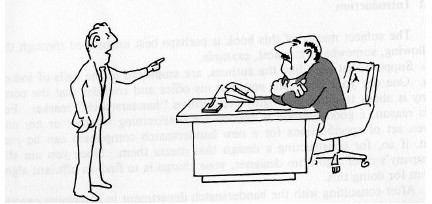
\includegraphics[width=0.55\textwidth]{images/chefe2.jpg}
	\end{center}
	\begin{itemize}
		\item A resposta mais forte, se fosse possível dá-la: provar que
			\textbf{nenhum} algoritmo eficiente pode existir para o
			problema;
		\item O obstáculo: isso exigiria provar $P \neq NP$ — uma questão
			em aberto há mais de 50 anos. Hoje, ninguém sabe como dar essa
			resposta.
	\end{itemize}
\end{frame}

\begin{frame}
	\frametitle{Resposta 3 --- ``Não consegui, mas ninguém mais também
		conseguiu''}
	\begin{center}
		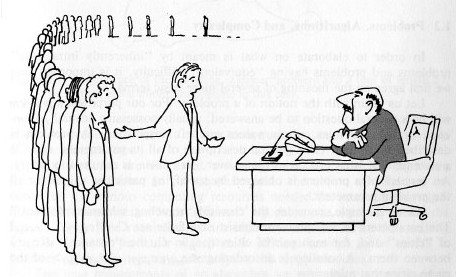
\includegraphics[width=0.6\textwidth]{images/chefe3.jpg}
	\end{center}
	\begin{itemize}
		\item A resposta praticável: mostrar que o problema é
			\textbf{NP-difícil} — está, comprovadamente, na companhia dos
			problemas mais difíceis que se conhece;
		\item Não prova que um algoritmo eficiente é impossível, mas
			mostra que encontrá-lo resolveria, de uma vez, todos os
			problemas de NP;
		\item É essa a resposta que o restante desta aula prepara vocês
			para dar.
	\end{itemize}
\end{frame}

\begin{frame}
	\frametitle{Uma limitação já observada}
	\begin{itemize}
		\item Na tarefa da Aula 5, a formulação MCF do TSP se tornou
			\textbf{impraticável} já nas instâncias maiores, por causa do
			crescimento $O(n^3)$ do número de variáveis de fluxo;
		\item Mesmo a formulação MTZ, mais compacta, pode não fechar o GAP
			dentro do tempo limite em instâncias maiores;
		\item O TSP é um problema de otimização combinatória — o número de
			rotas possíveis cresce como $(n-1)!/2$;
		\item Isso não é uma falha da formulação ou do solver: é uma
			propriedade do próprio problema — sua complexidade
			computacional intrínseca;
		\item Esta aula formaliza essa propriedade através dos conceitos
			de NP-dificuldade e da relação P \textit{versus} NP.
	\end{itemize}
\end{frame}

%------------------------------------------------------------
\section{Complexidade computacional}
%------------------------------------------------------------

\begin{frame}
	\frametitle{Instância de um problema}
	\begin{itemize}
		\item Um problema $P$ é definido por uma estrutura genérica de
			parâmetros;
		\item Uma \textbf{instância} $I$ de $P$ é uma atribuição concreta
			de valores a esses parâmetros;
		\item Exemplo — o Problema da Mochila:
	\end{itemize}
	$$
		\text{max}~\sum_{j=1}^{n}c_jx_j : \sum_{j=1}^{n}a_jx_j \leq b,~x \in
		B^n
	$$
	\begin{itemize}
		\item Uma instância fixa $n$, os coeficientes $c_j$, $a_j$ e o
			limite $b$.
	\end{itemize}
\end{frame}

\begin{frame}
	\frametitle{Tamanho de uma instância}
	\begin{itemize}
		\item O tamanho de uma instância $I$, denotado $L(I)$, é o
			comprimento da representação binária de seus dados de entrada;
		\item Para o Problema da Mochila:
	\end{itemize}
	$$
		L(I) = \sum_{j=1}^{n}\lceil \log_2 c_j \rceil + \sum_{j=1}^{n}
		\lceil \log_2 a_j \rceil
	$$
	\begin{itemize}
		\item É em função de $L(I)$ — não do número de variáveis isolado —
			que se mede o crescimento do esforço computacional.
	\end{itemize}
\end{frame}

\begin{frame}
	\frametitle{Tempo de execução de um algoritmo}
	\begin{itemize}
		\item Dado um problema $P$, um algoritmo $A$ para $P$ e uma
			instância $I$, seja $f_A(I)$ o número de operações elementares
			que $A$ realiza sobre $I$;
		\item A \textbf{função complexidade} $f_A^*(k)$ é o tempo de
			execução de $A$ no pior caso, entre todas as instâncias de
			tamanho $k$ — o asterisco distingue essa função (pior caso
			sobre um tamanho $k$) de $f_A(I)$ (tempo numa instância
			$I$ específica):
	\end{itemize}
	$$
		f_A^*(k) = \max_I \{f_A(I) : L(I) = k\}
	$$
\end{frame}

\begin{frame}
	\frametitle{Algoritmo eficiente}
	\begin{block}{Definição}
		$A$ é eficiente se existem um inteiro positivo $p$ e uma constante
		positiva $c$ tais que:
		$$
			f_A^*(k) \leq ck^p
		$$
	\end{block}
	\begin{itemize}
		\item Ou seja: o tempo de execução é limitado por um polinômio no
			tamanho da entrada.
	\end{itemize}
\end{frame}

\begin{frame}
	\frametitle{Algoritmo não eficiente}
	\begin{block}{Definição}
		Existem constantes $c_1, c_2 > 0$, $d_1, d_2 > 1$ e um inteiro
		$k'$ tais que, para todo $k \geq k'$:
		$$
			c_1 d_1^k \leq f_A^*(k) \leq c_2 d_2^k
		$$
	\end{block}
	\begin{itemize}
		\item Exemplos de crescimento exponencial:
		\begin{itemize}
			\item enumerar $2^k$ vetores binários de dimensão $k$;
			\item enumerar $n!$ permutações de $n$ elementos — a ordem de
				grandeza do número de rotas do TSP.
		\end{itemize}
	\end{itemize}
\end{frame}

%------------------------------------------------------------
\section{Problemas de busca e a classe NP}
%------------------------------------------------------------

\begin{frame}
	\frametitle{Problemas de decisão e problemas de busca}
	\begin{itemize}
		\item Formalmente, a teoria da complexidade define a classe NP
			sobre \textbf{problemas de decisão}: perguntas de resposta
			sim/não (ex.: ``existe uma rota de custo $\leq k$?'');
		\item Um problema de \textbf{otimização} (ex.: ``qual a rota de
			menor custo?'') tem uma versão de decisão associada: perguntar
			se existe solução de valor pelo menos tão bom quanto um limiar
			$k$ dado;
		\item Nesta disciplina, tratamos os dois sob o mesmo enfoque —
			\textbf{problema de busca}: dada uma solução candidata (ou um
			limiar $k$), verificar sua correção (ou se ela o alcança) em
			tempo polinomial.
	\end{itemize}
\end{frame}

\begin{frame}
	\frametitle{Problemas de busca}
	\begin{block}{Definição}
		Um problema de busca é aquele em que, dada uma solução candidata,
		é possível verificar sua correção em tempo polinomial.
	\end{block}
	\begin{itemize}
		\item A classe \textbf{NP} reúne todos os problemas de busca com
			essa propriedade;
		\item Verificar uma solução dada é, em geral, muito mais barato do
			que encontrá-la.
	\end{itemize}
\end{frame}

\begin{frame}
	\frametitle{Verificar é fácil, encontrar é difícil}
	\begin{itemize}
		\item O número $13.717.421$ pode ser escrito como o produto de
			dois outros inteiros. Quais?
	\end{itemize}
\end{frame}

\begin{frame}
	\frametitle{Verificar é fácil, encontrar é difícil}
	$$
		13.717.421 = 3.607 \times 3.803
	$$
	\begin{itemize}
		\item Multiplicar os dois fatores para conferir o resultado é
			imediato;
		\item Encontrá-los a partir só do produto é o difícil.
	\end{itemize}
\end{frame}

%------------------------------------------------------------
\section{P versus NP}
%------------------------------------------------------------

\begin{frame}
	\frametitle{As classes P e NP}
	\begin{itemize}
		\item \textbf{P}: problemas de busca resolvíveis em tempo
			polinomial por um algoritmo determinístico;
		\item \textbf{NP}: problemas de busca cuja solução, uma vez dada,
			pode ser verificada em tempo polinomial;
		\item $P \subset NP$: todo problema resolvível em tempo polinomial
			também tem suas soluções verificáveis em tempo polinomial.
	\end{itemize}
\end{frame}

\begin{frame}
	\frametitle{NP-completo e NP-difícil}
	\begin{itemize}
		\item \textbf{NP-completo}: problema em NP para o qual todo outro
			problema de NP pode ser reduzido em tempo polinomial;
		\item \textbf{NP-difícil}: pelo menos tão difícil quanto os
			problemas mais difíceis de NP — algum problema NP-completo pode
			ser reduzido para ele em tempo polinomial, mas ele mesmo não
			precisa estar em NP;
		\item Se um único problema NP-completo fosse resolvido em tempo
			polinomial, todos os problemas de NP também seriam — essa é a
			pergunta em aberto conhecida como P \textit{versus} NP.
	\end{itemize}
\end{frame}

\begin{frame}
	\frametitle{O primeiro problema NP-completo: SAT}
	\begin{itemize}
		\item \textbf{SAT} (satisfatibilidade booleana): dada uma fórmula
			lógica com variáveis booleanas, existe alguma atribuição de
			verdadeiro/falso às variáveis que torna a fórmula inteira
			verdadeira?
		\item \textbf{Teorema de Cook--Levin} (Cook, 1971; Levin, 1973,
			de forma independente): SAT é NP-completo;
		\item Foi o \textbf{primeiro} problema provado NP-completo — e por
			isso não podia ser provado por redução a partir de outro
			NP-completo (não existia nenhum ainda). A prova simula
			diretamente a execução de qualquer máquina não-determinística
			polinomial como uma fórmula booleana;
		\item A partir de SAT, Karp (1972) provou outros 21 problemas
			NP-completos por redução — inaugurando a técnica do próximo
			slide.
	\end{itemize}
\end{frame}

\begin{frame}
	\frametitle{Por que basta reduzir um NP-completo conhecido}
	\begin{itemize}
		\item A definição formal de NP-difícil exige que \textbf{todo}
			problema de NP se reduza a ele — na prática, ninguém verifica
			isso um a um;
		\item Basta reduzir, em tempo polinomial, um \textbf{único}
			problema $Y$ já conhecido como NP-completo (ex.: SAT, ou algum
			dos 21 de Karp) para o problema $X$ que se quer classificar
			($Y \leq_p X$);
		\item Isso basta por \textbf{transitividade}: como $Y$ é
			NP-completo, todo $L \in NP$ já se reduz a $Y$ ($L \leq_p Y$);
			encadeando as duas reduções, $L \leq_p X$ para todo $L \in
			NP$ — ou seja, $X$ também é NP-difícil;
		\item É essa técnica — reduzir um problema conhecido para o novo
			problema — que se usa na prática para provar NP-dificuldade,
			desde o SAT em diante.
	\end{itemize}
\end{frame}

\begin{frame}
	\frametitle{P, NP, NP-completo e NP-difícil — se $P \neq NP$}
	\begin{center}
	\begin{tikzpicture}[scale=0.9]
		\draw[thick] (0,0) ellipse (4.4 and 2.6);
		\node at (0,2.15) {NP};
		\draw[thick] (-2.3,-0.4) ellipse (1.6 and 1.2);
		\node at (-2.3,-0.4) {P};
		\draw[thick] (1.9,0.1) ellipse (1.7 and 1.7);
		\node at (1.9,1.35) {NP-completo};
		\draw[thick,dashed] (3.0,-1.7) ellipse (2.6 and 1.4);
		\node at (4.0,-2.5) {NP-difícil};
	\end{tikzpicture}
	\end{center}
	\begin{itemize}
		\item Cenário \textbf{conjecturado} (não provado): P e
			NP-completo aparecem como conjuntos disjuntos dentro de NP;
		\item NP-difícil se estende além de NP (por isso o contorno
			tracejado): inclui também problemas que não são, eles mesmos,
			problemas de decisão/busca verificáveis em NP.
	\end{itemize}
\end{frame}

\begin{frame}
	\frametitle{P, NP, NP-completo e NP-difícil — se $P = NP$}
	\begin{center}
	\begin{tikzpicture}[scale=0.68]
		\draw[thick] (0,0) ellipse (3.1 and 2.4);
		\node at (0,1.75) {P $=$ NP};
		\draw[thick] (0.5,-0.3) ellipse (1.7 and 1.4);
		\node at (0.5,-0.3) {NP-completo};
		\draw[thick,dashed] (2.7,-1.8) ellipse (2.6 and 1.4);
		\node at (3.7,-2.6) {NP-difícil};
	\end{tikzpicture}
	\end{center}
	\begin{itemize}
		\item Se P $=$ NP, os problemas NP-completos passam a estar
			também em P: resolvíveis em tempo polinomial;
		\item A definição de NP-completo/NP-difícil não muda — continuam
			sendo os problemas para os quais todo NP se reduz —, mas eles
			deixam de representar uma dificuldade genuinamente maior que a
			de P;
		\item NP-difícil continua se estendendo além de NP: essa parte não
			depende de P \textit{versus} NP ser verdadeiro ou falso.
	\end{itemize}
\end{frame}

\begin{frame}
	\frametitle{Voltando à resposta 3}
	\begin{itemize}
		\item Mostrar que o TSP é NP-difícil é exatamente a resposta 3
			da motivação: reduzir um problema já conhecido como
			NP-completo para o TSP, em vez de provar do zero;
		\item Isso não é desculpa vaga — é uma demonstração formal de
			que o problema está entre os mais difíceis que se conhece;
		\item É essa demonstração que torna tecnicamente aceitável não
			ter resolvido a instância até a otimalidade, sem que isso seja
			incompetência de quem programou.
	\end{itemize}
\end{frame}

\begin{frame}
	\frametitle{Reflexão}
	\begin{itemize}
		\item Grande parte dos problemas de otimização combinatória de
			interesse prático — entre eles o TSP — é NP-difícil;
		\item Isso não impede o uso de formulações exatas: em instâncias
			pequenas ou moderadas, um solver resolve o problema até a
			otimalidade comprovada;
		\item Mas, para instâncias grandes, o tempo e a memória necessários
			podem simplesmente inviabilizar a abordagem exata;
		\item É nesse cenário que entram as heurísticas.
	\end{itemize}
\end{frame}

%------------------------------------------------------------
\section{Heurísticas}
%------------------------------------------------------------

\begin{frame}
	\frametitle{Etapas da resolução de um problema de otimização}
	\begin{itemize}
		\item Formulação do problema;
		\item Análise do problema formulado;
		\item Delimitação das restrições de aplicação: tempo disponível,
			memória disponível, qualidade de solução exigida;
		\item Escolha do método de resolução apropriado a essas restrições.
	\end{itemize}
\end{frame}

\begin{frame}
	\frametitle{Heurística}
	\begin{block}{Definição}
		Técnica que busca alcançar uma solução de boa qualidade com um
		esforço computacional considerado razoável, sem garantir, em
		geral, nem a otimalidade nem — dependendo do método — sequer a
		viabilidade da solução encontrada.
	\end{block}
	\begin{itemize}
		\item Em troca da garantia de otimalidade, ganha-se velocidade;
		\item É essa a troca que justifica seu uso quando o solver exato
			não é uma opção viável.
	\end{itemize}
\end{frame}

\begin{frame}
	\frametitle{Heurística construtiva}
	\begin{itemize}
		\item Constrói uma solução viável do zero, sem partir de uma
			solução anterior;
		\item Objetivos desejáveis: solução de boa qualidade e custo
			computacional baixo;
		\item Exemplos:
		\begin{itemize}
			\item construção aleatória;
			\item construção gulosa;
			\item resolver uma relaxação do problema e arredondar a
				solução;
			\item outros.
		\end{itemize}
	\end{itemize}
\end{frame}

%------------------------------------------------------------
\section{Duas heurísticas construtivas para o TSP}
%------------------------------------------------------------

\begin{frame}
	\frametitle{Representação de uma solução do TSP}
	\begin{itemize}
		\item Uma rota pode ser representada por um array com a sequência
			de cidades visitadas, por exemplo $\{1, 2, 4, 6, 7, 3, 5, 1\}$;
		\item O custo da solução é a soma das distâncias entre cidades
			consecutivas na sequência, incluindo o retorno à origem;
		\item Toda heurística construtiva para o TSP produz, ao final, uma
			sequência desse tipo.
	\end{itemize}
\end{frame}

\begin{frame}
	\frametitle{Construção aleatória}
	\begin{itemize}
		\item Gera uma permutação aleatória das cidades como rota;
		\item Não usa nenhuma informação sobre as distâncias entre
			cidades;
		\item A qualidade da solução obtida é uma questão de sorte —
			resultados muito distintos entre execuções são esperados;
		\item Custo computacional mínimo: gerar a permutação e calcular o
			custo.
	\end{itemize}
\end{frame}

\begin{frame}
	\frametitle{Heurística do vizinho mais próximo}
	\begin{itemize}
		\item Parte de uma cidade de origem;
		\item Em cada passo, vai para a cidade não visitada mais próxima
			da cidade atual;
		\item Repete até visitar todas as cidades, e então retorna à
			origem;
		\item Usa a informação de distância a cada passo — diferente da
			construção aleatória;
		\item Não garante que a rota gerada seja ótima: uma escolha
			gulosa no início pode forçar um deslocamento longo mais tarde;
		\item Pode ser repetida a partir de cada cidade de origem
			possível, guardando a melhor rota entre todas as partidas.
	\end{itemize}
\end{frame}

%------------------------------------------------------------
\section{A tarefa (avaliativa)}
%------------------------------------------------------------

\begin{frame}
	\frametitle{Caráter avaliativo}
	\begin{itemize}
		\item Esta tarefa vale \textbf{25\% da nota da Unidade 1};
		\item Pode ser realizada em equipes de até 3 pessoas;
		\item Retoma as quatro instâncias e os ótimos conhecidos já usados
			na tarefa da Aula 5 (\texttt{berlin52}, \texttt{kroA100},
			\texttt{ch150}, \texttt{kroA200}).
	\end{itemize}
\end{frame}

\begin{frame}
	\frametitle{O que é pedido}
	\begin{itemize}
		\item Implementar a heurística do vizinho mais próximo, em duas
			variantes: partindo só da cidade 1, e multi-start (a partir de
			cada cidade, guardando a melhor);
		\item Implementar a construção aleatória, com 30 execuções por
			instância, reportando custo médio, desvio-padrão, melhor custo
			e tempo;
		\item Montar uma tabela de resultados, uma linha por instância,
			comparando as três heurísticas diretamente com o ótimo
			conhecido;
		\item Descrever o ambiente computacional usado — processador,
			memória, sistema operacional, linguagem, solver e número de
			threads.
	\end{itemize}
\end{frame}

%------------------------------------------------------------
\section{Referências}
%------------------------------------------------------------

\begin{frame}
	\frametitle{Referências}
	\begin{itemize}
		\item Garey, M. R.; Johnson, D. S. \textit{Computers and
			Intractability: A Guide to the Theory of NP-Completeness}.
			1979. (fonte das ilustrações das três respostas possíveis)
		\item Goldbarg, M. C.; Luna, H. P. L. \textit{Otimização
			Combinatória e Programação Linear}. 2005.
		\item Hillier, F. S.; Lieberman, G. J. \textit{Introduction to
			Operations Research}. 2010.
		\item Cook, S. A. The complexity of theorem-proving procedures.
			\textit{Proceedings of the 3rd Annual ACM Symposium on Theory
			of Computing (STOC)}, 1971.
		\item Karp, R. M. Reducibility among combinatorial problems. In:
			\textit{Complexity of Computer Computations}, 1972.
		\item Miller, C. E.; Tucker, A. W.; Zemlin, R. A. Integer
			programming formulation of traveling salesman problems.
			\textit{Journal of the ACM}, 1960.
	\end{itemize}
\end{frame}

\end{document}
